\documentclass[a4paper, 10pt]{article}
\usepackage{xcolor}
\usepackage{graphicx}
\usepackage[colorlinks=true, linkcolor=blue, urlcolor=blue]{hyperref}

\title{The Lure of Emerging Virtual Computers}

\author{Reza Hasanzadeh\thanks{This work has been funded by a generous grant from the \href{https://www.ethswarm.org
}{Swarm Assosiation}.}  \\ \href{mailto:rezahsnz@proton.me}{\small{rezahsnz@proton.me}}}

\date{\small{Draft} \\ \small{November 30th, 2022}}

\begin{document}

\definecolor{fairgreen}{rgb}{0, 0.3, 0.15}

\maketitle

\section{Introduction}

\section{Primordial soup}

\subsection{Swarm and FairOS-DFS}
\textbf{Swarm}\footnote{\url{https://www.ethswarm.org}} is network of peer-to-peer nodes(computers) joined together to form a unified  information storage and communication facility. Storage involves dividing data into small chunks(usually 4KB in size) and distributing them over the whole network in a way that retrieval is also quick. Each chunk ends up being stored on different node(s) to ensure resiliency against single node failures. Each File is addressed using the hash value resulting from its \texttt{Balanced Merkle Tree} representation. This storage and addressing shceme is commonly known as \texttt{content addressing} which in essence eliminates the need for extra metadata about the location of the stored data with the added benefit of robust integrity checks. To store data, one needs to buy the rights to write into the storage space. The medium of exchange within the Swarm network is called the BZZ token. This token acts as the incentive paid to the storage providers in return for their physical contributions to the netwok. This properly-incentivized, resilient, and privacy-respecting setup paves the way for more abrstract interfaces to appear.
\par \noindent 
Swarm's interface, though sophisticated, is still clumsy for humane uses. This is where \textbf{FairOS-DFS} comes to rescue by introducing advanced interfaces that allow a rich basket of applications to be created in a shorter amount of spacetime. Figure  \ref{swarmfair} demonstrates the relationship between Swarm and FairOS-DFS and the set of interfaces available for application developers\footnote{\url{https://docs.fairos.fairdatasociety.org/docs/fairOS-dfs/introduction}}. As is seen on the figure almost all the storage related functionalities are baked into the DFS layer. Out of all of them, the function of the \texttt{pod} seems to be very handy. Pods are operated just like any regular local device on a unix-like operating system. Pods play a central rule within the DFS layer where most write/read operations first need a pod to exist and be accessible. This umbrella scheme of pods let even more abstract objects to appear on top of DFS. If an application is a directory structure, for example, then each application can be stored on Swarm as an standalone pod. Pods can communicate with one another through sharing parts(e.g. a file within the pod) or all of the pod with the outside world. The identification of pods are done through their \texttt{names} with no two pods sharing the same name within a user's wallet. Pods are private to each user unless she decides to make it available to the outside world. This is done through a sharing mechanism. Once a pod(or a file within it) is shared, a \texttt{reference key} is generated that allows others to get a copy of the pod. Though simple, this notion of the pod enables a rich league of inteacting objects to be sowed on the fertile soil of Swarm lands where the emergence of a \textit{brave new world} of virtual computers is inevitable.

\begin{figure}
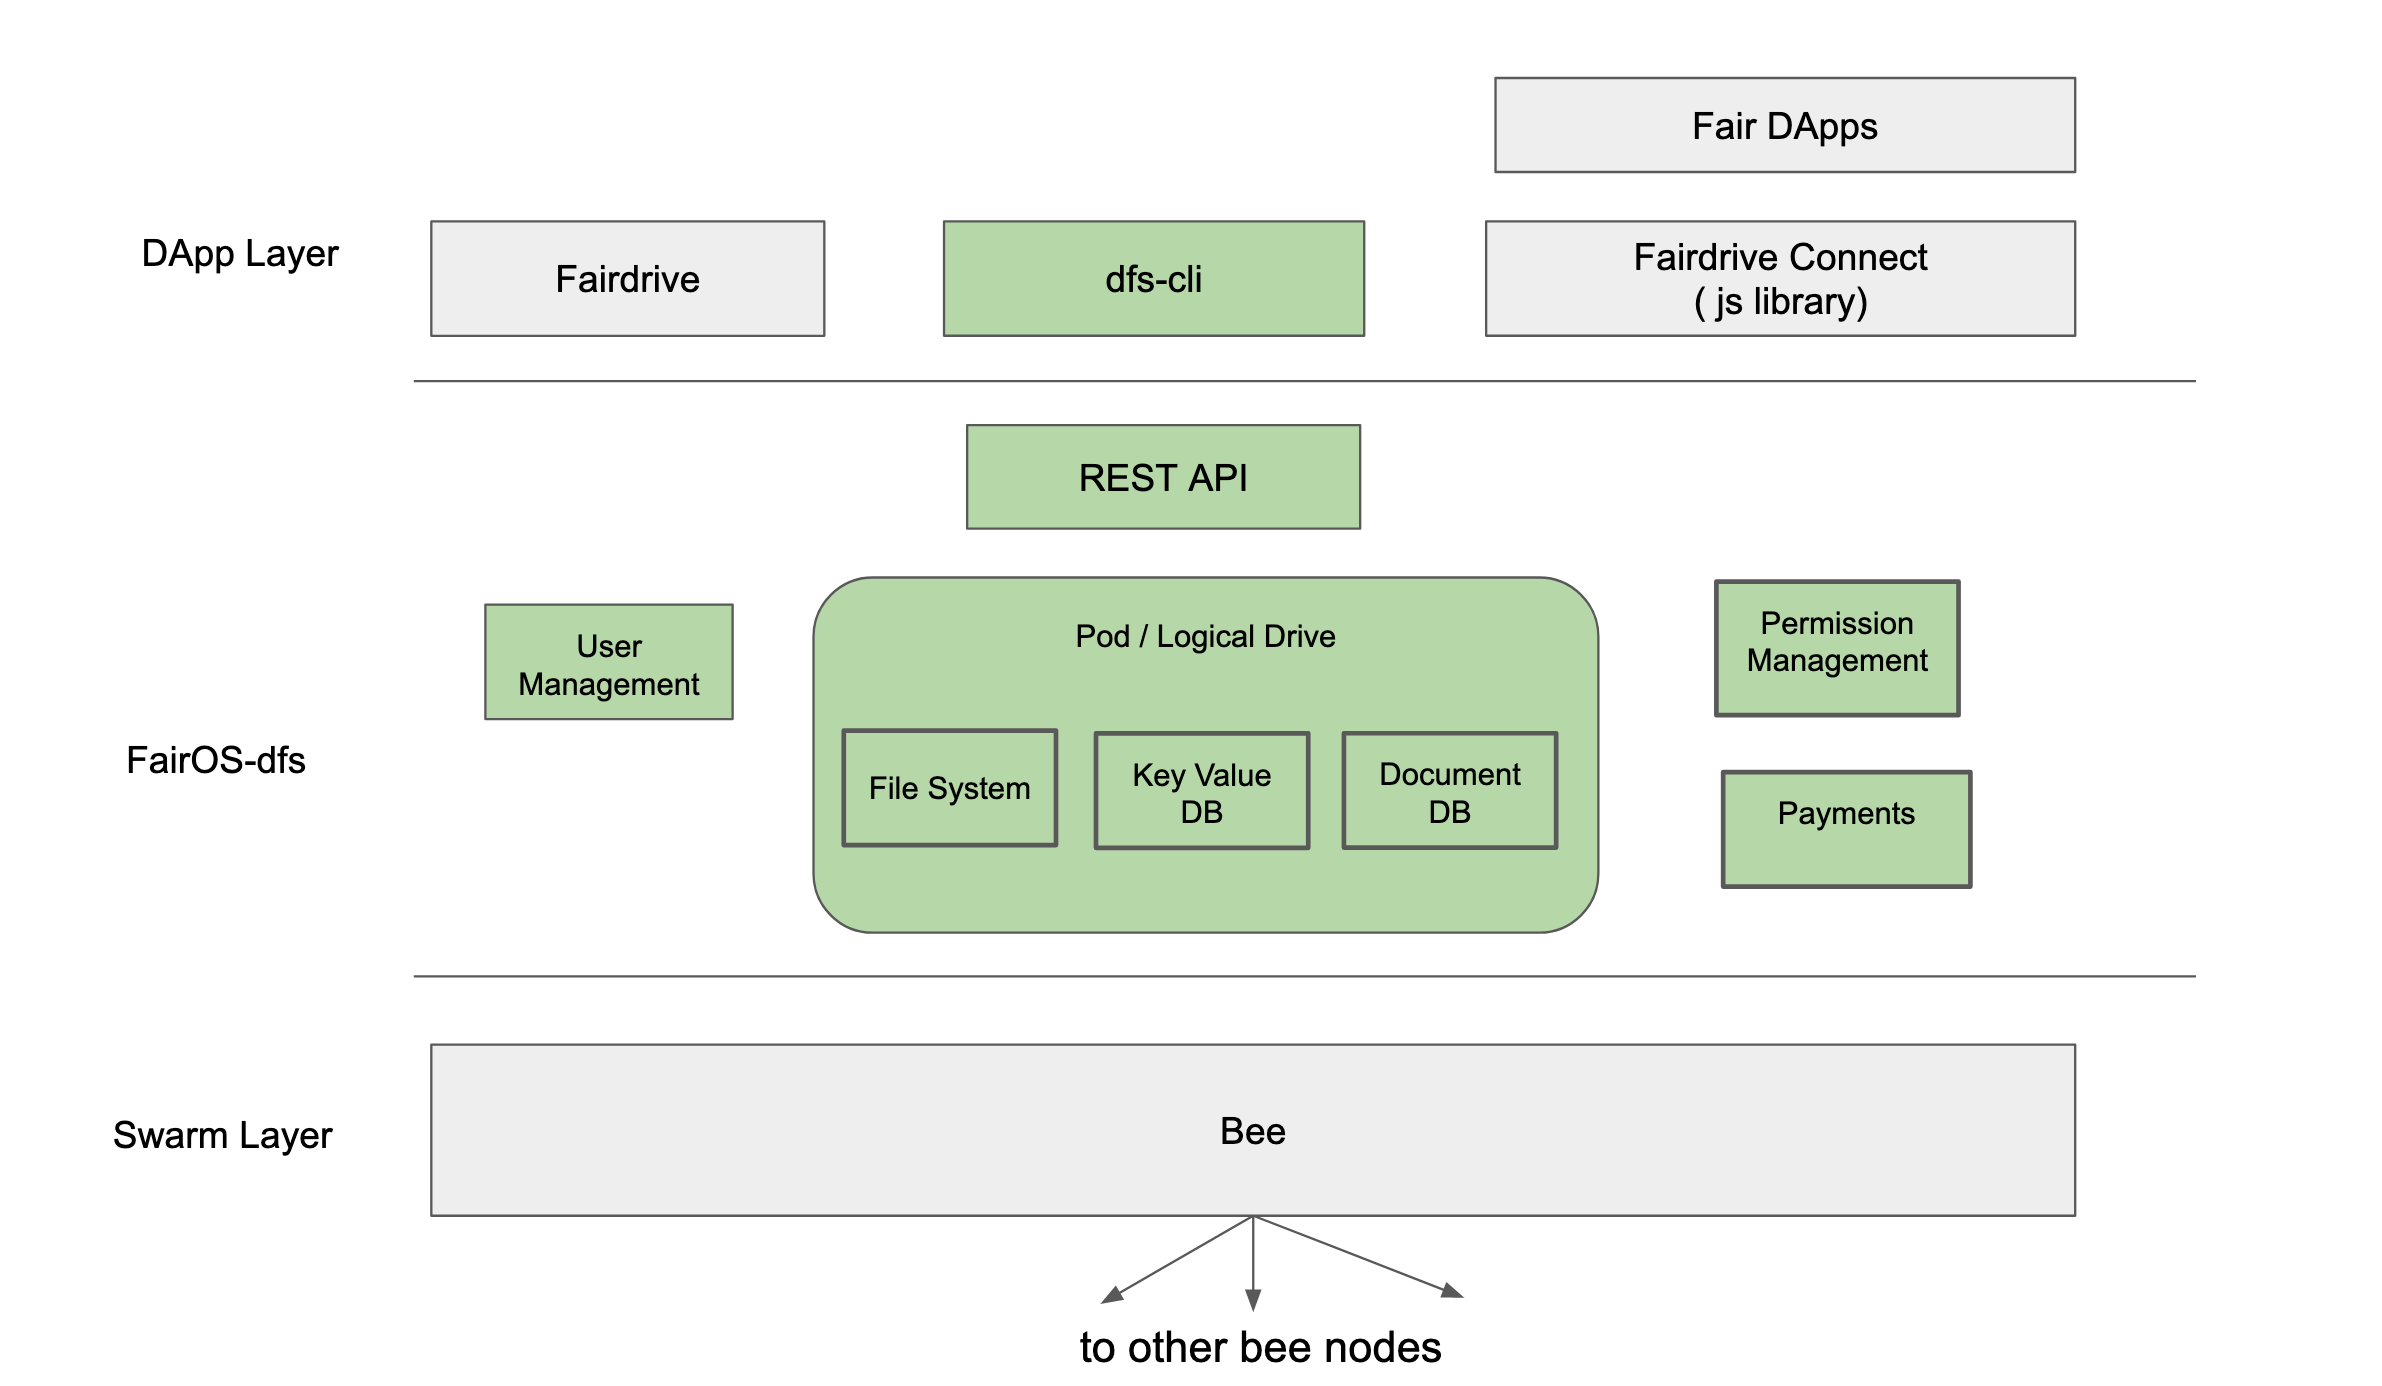
\includegraphics[scale=0.3,keepaspectratio=true]{images/swarm-fair.png}
\caption{\label{swarmfair}Swarm and \textcolor{fairgreen}{FairOS-DFS}}
\end{figure}

\subsection{Golem network}
\textbf{Golem network}\footnote{\url{https://www.golem.network}} is a peer-to-peer marketplace for compute jobs. It consists of three entities: \texttt{requestors} who need and pay for compute resources(cpu, ram , ...), \texttt{providers} who offer their compute resources in exchange for money, and a matching agent called the \texttt{YAGNA daemon} that mediates between requestors and providers. A compute job is initiated by a requestor who makes a demand specifying the minimum amount of resources(e.g. 24GB of ram) needed along with the budget in GLM\footnote{GLM is an ERC-20 token and the medium of exchange within the Golem network.} and waits for any provider to accept her criteria. Once an aggrement is reached, the provider loads the execution environment(a golemized-docker image already prepared and registered within the Golem network) and starts running the job. When the execution of the job is finished, the requestor collects the output (and any logs) and pays for the services she has used. The following three sections briefly describe the important participants of the Golem network.
\subsubsection*{Requestors}
Requestor is an umbrella term for a set of agents working together to make a compute job happen. Golem network operates on the Ethereum network with support for other EVM-compatible blockchain like the Polygon network. The first step for a requestor is to have a valid wallet loaded with enough funds to sign transactions and pay the compute bills. Then comes the need to prepare an execution environment within which the logic of the compute job is going to be carried out. This environment is a Docker image that will be started by providers once an agreement is reached. This image first needs to be golemized and added to the Golem's image registry. Then comes the actual logic of a compute job: a set of Python\footnote{Support for Javascript code is also provided} files, data files, and shell scripts that manage the compute job. File exchange channels brought up by YAGNA allows a requestor to send any files to the execution environment. These exchanges can happen from the start of the job all through the end of it, first sending data and code and then collecting outputs and logs. Once the compute job is finished, the bill is ready to be paid.
\subsubsection*{Providers}
A provider is simply a fraction of a computer's resources that is ready to be used within the marketplace set up by the Golem network. Just like the requestors, providers use the channels relayed by the YAGNA daemon(s) for communicating with other network participants. A provider needs a wallet, some virtualized-ready operating system services, and a fraction of the resources to serve requestors. Providers often publish their offers in response to demands advertised on the network and when the agreement is reached, they start doing the job and get paid for it. Recall that the medium of exchange in Golem network is GLM and the rates are denominated in GLM/hour. Providers can change rates anytime and this flexibility is a double-edged feature: set rates too high and no one would be interested in your services, set them too low and you risk being unable to pay electricity bills. This is exacerbated by the volatile nature of the GLM token as the price of GLM is subject to market conditions. 
\subsubsection*{The mediator}
Golem network is a peer-to-peer marketplace for compute jobs. A demand for a compute job is first published on the network and then offers are collected from providers. A typical offer includes a proposal that contains the specs of the hardware along with the rates for services. Of all offers received, the least expensive one is usually chosen and agreed with though this strategy can be changed through the requestor code. Once an agreement is reached, the budget for this job is locked by the YAGNA and when the job is finished, gets transferred to the provider. The YAGNA daemon mediates these communications between providers and requestors. The requestor's side of the mediation is composed of the YAGNA HTTP server along with client toolkits in the form of Python and Javascript libraries for communicationg with the HTTP server. The provider's side of mediation too consists of a daemon that waits for incoming demands, makes proposals to requestors, and manages all wallet related tasks.

\section{Emergence of computers}

\subsection{Compute pods and the Sovr protocol}

\subsubsection*{Communications}

\subsection{Decentralised compute}

\subsubsection*{Self-regulating computers}

\end{document}
